%!TEX root = ../Master.tex
\section{Mesurement methods}\label{sec:measure}

This section contains the descriptions and methods of the tests conducted, in order to understand how and when the different reliability mechanisms should be adapted.
To simplify our analysis we make the assumption that the sender has perfect feedback and is able to switch TxR, RLNC and video rate instantaneously. At the receiver we assume no delay is caused by feedback, erasure coding or the video player, and we assume that all receivers receive the same throughput from the sender. Additionally, we assume that RLNC introduces no data overhead or linear dependency. Finally, the throughput examination assumes that every receiver's link to the drone is identical. Based on these assumptions only the channel condition has an effect on the system delay and we model the system as two queues, see Figure \ref{fig:buffer}. 
\begin{figure}[ht]
  \centering
  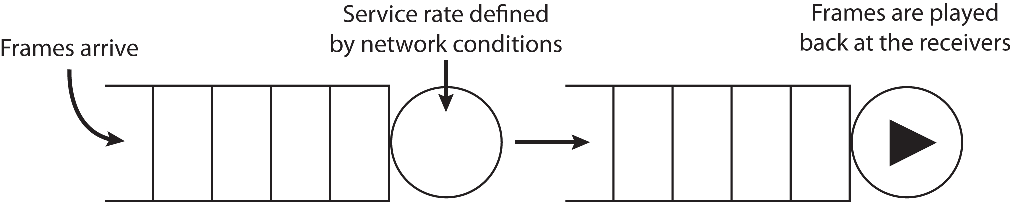
\includegraphics[width=\linewidth]{images/SimpleSystem.pdf}
  \caption{Simplified system model}
  \label{fig:buffer}
\end{figure}

When a frame is captured by the drone at a given video rate it is prepared for transmission with additional redundancy. Packets are placed in a buffer and serviced sequentially based on the capability of the transmitting network. When a packet is serviced it is transferred instantaneously to the receivers playback-buffer and ready to be serviced by the receivers video player.

All the tests are performed using the same test equipment. A receiver consist of one Raspberry Pi 1 model B and a TP-link TL-WN722N USB WiFi dongle. The sender is a Raspberry Pi 3 model B which uses the WiFi dongle RT5370. Both the sender and receivers are running Raspbian linux. The sender is configured as an 802.11g access point\cite{IEEE80211g}. The drone used to carry the sender is a Parrot Bebop 2 drone.

Unless otherwise stated the empirical tests are performed with one sender and 4 receivers, where the receivers are placed right next to each other. Multiple receivers are used to account for hardware diversity.
\subsection{TxR}
To understand how the different TxR perform in practice when comparing to the physical location of the drone, we measure the percentage of UDP packets reaching a receiver as a function of the distance and height between sender and receiver.
% How
We conduct a number of tests, varying one parameter at a time. Each test has a duration of 1 minute.
The different bit rates tested were 12, 18, 24, 36 megabit per second (Mb/s) at distances between 10 and 100 m, in 10 m intervals at a height of 45 cm and 2 m. For each TxR we measure the UDP SDU throughput at the sender in order to determine the actual data rate available for the video data.
\subsection{Video rates}
% What - Do we want to test?
In order to understand the behaviour of different video rates, we analyse videos obtained from the drone using VBR \cite{WorksheetH264}. The target bitrates are set to 5, 10, 20 Mb/s and a large open area is recorded. To perform the analysis of the video, petro\cite{petro} (a video analysis tool) has been used.
\subsection{Aerial data collection}\label{subsec:ArealData}
For the main source of analysis we use the drone in the scenario previously described in Section \ref{sec:methodmaterials} to obtain a trace which shows the packet loss at each TxR simultaneously \cite{droneVid}. The sender can only transmit at one rate at a time. Therefore, the following technique is used to estimate the continues channel behaviour for each TxR: the sender alternates between the four rates 12, 18, 24, 36 Mb/s, sending 20 packets at each rate before switching. Since TxR is changed from user space, we include a delay to ensure packets are send with the correct TxR.
The time to send one packet (denoted $ t_{s} $) depends on the TxR. The slowest rate is 12 Mb/s and assuming a packet size of 1500 B, each packet takes approximately 1 ms to send, as seen in equation \ref{eq:tts}.
\begin{equation}
	\begin{split}
		t_{s} \approx  \frac{8 \frac{b}{B} \cdot 1500 \ B}{12 \ Mb/s}  =  \frac{12 \ kb}{12 \ Mb/s} = 1 \ ms
	\end{split}
	\label{eq:tts}
\end{equation}
This delay is used for all rates to simplify data analysis. Empirical experiments have shown that adding 5 ms to $ 20 \cdot t_{s} $ gives a sufficiently large certainty, that all the packets have been sent.
Therefore, the sender transmit 20 packets, wait 25 ms, adjust TxR and repeat. This means that out of 100 ms, at most $1/4$ of the time is used to transmit at one rate. We use the drop rate of the 20 packets to estimate the channel behaviour in the rest of the time interval.
We show in \cite{WorksheetValidEstimate} that this estimate is in fact valid and gives a good representation of the true application layer throughput.

%We analyse the playback delay and buffer requirements imposed on the system by the different video streams, with the collected network trace. We choose the best possible data trace, i.e. we assemble the best rates at any given time, and use that to service the video data. The different data rates are analysed individually to see what the per frame delay and maximum buffer size requirements are.
